\documentclass[11pt,a4paper]{article}
\usepackage[utf8]{inputenc}
\usepackage[T1]{fontenc}
\usepackage{lmodern}
\usepackage[portuguese]{babel}
\usepackage[a4paper,margin=2.4cm]{geometry}
\usepackage{xcolor}
\usepackage{graphicx}
\usepackage{titlesec}
\usepackage{enumitem}
\usepackage{listings}
\usepackage{tcolorbox}
\usepackage{booktabs}
\usepackage{amsmath}
\usepackage{amssymb}
\usepackage{fancyhdr}
\usepackage{hyperref}
\tcbuselibrary{skins,breakable,listings}

\definecolor{BgCream}{HTML}{FAF8F5}
\definecolor{TextEspresso}{HTML}{4A4238}
\definecolor{NudeTaupe}{HTML}{BFAFA6}
\definecolor{SoftBlush}{HTML}{D9C5B2}
\definecolor{SageMuted}{HTML}{7E8F7C}
\definecolor{ClayWarn}{HTML}{B5795C}

\hypersetup{colorlinks=true, linkcolor=TextEspresso, urlcolor=TextEspresso}

\titleformat{\section}{\color{TextEspresso}\Large\bfseries}{\thesection}{0.6em}{}[{\color{NudeTaupe}\titlerule[0.8pt]}]
\titleformat{\subsection}{\color{TextEspresso}\large\bfseries}{\thesubsection}{0.6em}{}
\titlespacing*{\section}{0pt}{1.4\baselineskip}{0.7\baselineskip}
\titlespacing*{\subsection}{0pt}{1.1\baselineskip}{0.5\baselineskip}

\lstset{
  basicstyle=\ttfamily\small,
  breaklines=true,
  columns=fullflexible,
  showstringspaces=false,
  frame=none,
  aboveskip=0pt, belowskip=0pt
}

\pagestyle{fancy}
\fancyhf{}
\renewcommand{\headrulewidth}{0pt}
\fancyfoot[C]{\color{NudeTaupe}\small\thepage}

% ---- Caixa: comandos a executar ----
\newtcblisting{terminal}{
  listing only, breakable,
  colback=BgCream, colframe=NudeTaupe,
  boxrule=0.5pt, arc=2pt, left=6pt, right=6pt, top=5pt, bottom=5pt,
  listing options={basicstyle=\ttfamily\small, breaklines=true, columns=fullflexible}
}

% ---- Caixa: saida esperada ----
\newtcblisting{saida}{
  listing only, breakable,
  colback=white, colframe=SoftBlush,
  boxrule=0.5pt, arc=2pt, left=6pt, right=6pt, top=5pt, bottom=5pt,
  title={\small\bfseries\color{TextEspresso}Saída esperada},
  coltitle=TextEspresso, colbacktitle=SoftBlush!45,
  fonttitle=\small\bfseries,
  listing options={basicstyle=\ttfamily\footnotesize, breaklines=true, columns=fullflexible}
}

% ---- Caixa: ponto de verificacao ----
\newtcolorbox{verificar}{
  breakable, colback=SageMuted!8, colframe=SageMuted,
  boxrule=0.6pt, arc=2pt, left=7pt, right=7pt, top=6pt, bottom=6pt,
  title={\small\bfseries Confirme antes de avançar},
  coltitle=white, colbacktitle=SageMuted, fonttitle=\small\bfseries
}

% ---- Caixa: aviso ----
\newtcolorbox{atencao}{
  breakable, colback=ClayWarn!8, colframe=ClayWarn,
  boxrule=0.6pt, arc=2pt, left=7pt, right=7pt, top=6pt, bottom=6pt,
  title={\small\bfseries Atenção},
  coltitle=white, colbacktitle=ClayWarn, fonttitle=\small\bfseries
}

% ---- Caixa: nota/contexto ----
\newtcolorbox{nota}{
  breakable, colback=NudeTaupe!10, colframe=NudeTaupe,
  boxrule=0.5pt, arc=2pt, left=7pt, right=7pt, top=6pt, bottom=6pt
}

% ---- Cabecalho do manual ----
\newcommand{\manualtitle}[3]{%
  \thispagestyle{empty}
  \begin{center}
  {\color{NudeTaupe}\rule{\textwidth}{0.5pt}}\\[0.5cm]
  {\LARGE\bfseries\color{TextEspresso} Manual Técnico #1}\\[0.35cm]
  {\large\color{TextEspresso} #2}\\[0.3cm]
  {\normalsize\color{NudeTaupe} Infraestruturas de Computação na Nuvem \quad|\quad #3}\\[0.4cm]
  {\color{NudeTaupe}\rule{\textwidth}{0.5pt}}
  \end{center}
  \vspace{0.4cm}
}

% ---- Entrada de troubleshooting ----
\newcommand{\problema}[1]{\vspace{0.35cm}\noindent{\bfseries\color{TextEspresso}#1}\par\nopagebreak\vspace{0.1cm}}

\setlist[itemize]{itemsep=0.22cm, topsep=0.2cm}
\setlist[enumerate]{itemsep=0.22cm, topsep=0.2cm}

\begin{document}
\manualtitle{12}{Monitorização com Net-SNMP}{Aula 12}

\section*{Como usar este manual}

Vai montar a arquitetura clássica de gestão: uma máquina \emph{agente} expõe informação, outra \emph{manager} consulta-a. Depois vai capturar o tráfego e ver, com os seus próprios olhos, porque é que o SNMPv2c é considerado inseguro -- e o que o SNMPv3 muda.

\begin{atencao}
\textbf{Configure o SNMP apenas nas suas VMs.} Não instale nem altere nada no servidor Proxmox: é partilhado por toda a turma.
\end{atencao}

Os blocos indicam onde correr cada comando:
\begin{itemize}
  \item \textbf{[AG]} -- na VM agente (a máquina gerida)
  \item \textbf{[MG]} -- na VM manager (quem consulta)
\end{itemize}

\section*{Antes de começar}

\begin{center}
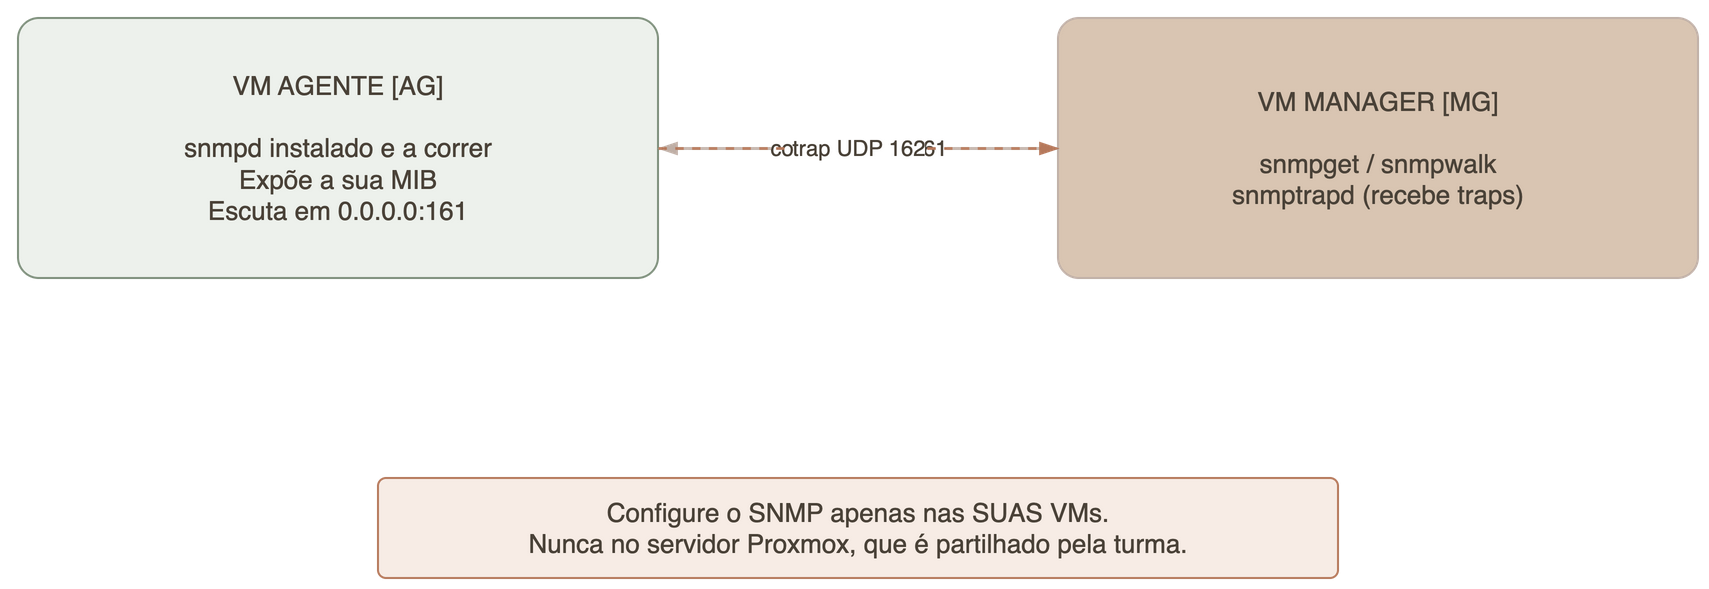
\includegraphics[width=\linewidth]{../Diagramas/m12-duas-vms.png}\\[0.15cm]
{\small\color{NudeTaupe} Uma VM faz de agente, outra de manager. Nunca o servidor Proxmox.}
\end{center}


\begin{itemize}
  \item[$\square$] Duas VMs ligadas, na mesma rede
  \item[$\square$] IPs registados
  \item[$\square$] Acesso \texttt{sudo} em ambas
\end{itemize}

\begin{terminal}
IP do agente  : ____.____.____.____
IP do manager : ____.____.____.____
\end{terminal}

\section{Instalar}

\textbf{[AG]}
\begin{terminal}
$ sudo apt update
$ sudo apt install -y snmpd
\end{terminal}

\textbf{[MG]}
\begin{terminal}
$ sudo apt update
$ sudo apt install -y snmp snmp-mibs-downloader snmptrapd
\end{terminal}

\section{Configurar o agente}

\textbf{[AG]}
\begin{terminal}
$ sudo cp /etc/snmp/snmpd.conf /etc/snmp/snmpd.conf.bak
$ sudo nano /etc/snmp/snmpd.conf
\end{terminal}

Duas alterações necessárias.

\subsection{Escutar na rede, não só localmente}

Por omissão, muitas distribuições limitam o agente a \texttt{127.0.0.1}. Procure a linha \texttt{agentaddress} e deixe-a assim:

\begin{terminal}
agentaddress udp:161
\end{terminal}

\begin{atencao}
Se ficar \texttt{agentaddress 127.0.0.1,[::1]}, o agente só responde a si próprio e todas as consultas do manager falharão por \emph{timeout}. É a causa número um de problemas nesta aula.
\end{atencao}

\subsection{Definir a community string e a vista}

Comente as linhas \texttt{rocommunity} existentes e acrescente (ajustando a sub-rede):

\begin{terminal}
rocommunity icnturma 192.168.1.0/24
view   systemonly  included   .1.3.6.1.2.1
\end{terminal}

\subsection{Reiniciar e confirmar}

\textbf{[AG]}
\begin{terminal}
$ sudo systemctl restart snmpd
$ sudo systemctl enable snmpd
$ sudo ss -lnup | grep 161
\end{terminal}

\begin{saida}
UNCONN 0  0   0.0.0.0:161   0.0.0.0:*   users:(("snmpd",pid=2841,fd=8))
\end{saida}

\begin{verificar}
Aparece \texttt{0.0.0.0:161} e não \texttt{127.0.0.1:161}. Se aparecer o segundo, volte ao \texttt{agentaddress}.
\end{verificar}

\section{Consultar a partir do manager}

\subsection{Uptime do sistema}

\textbf{[MG]}
\begin{terminal}
$ snmpget -v2c -c icnturma <IP-do-agente> 1.3.6.1.2.1.1.3.0
\end{terminal}

\begin{saida}
DISMAN-EVENT-MIB::sysUpTimeInstance = Timeticks: (184523) 0:30:45.23
\end{saida}

\begin{nota}
O OID \texttt{1.3.6.1.2.1.1.3.0} decompõe-se assim: \texttt{1.3.6.1} é \texttt{iso.org.dod.internet}; \texttt{.2.1} é a MIB-II; \texttt{.1} é o grupo \texttt{system}; \texttt{.3} é o \texttt{sysUpTime}; o \texttt{.0} final indica que é um valor único, não uma tabela.
\end{nota}

\subsection{Tabela de interfaces}

\textbf{[MG]}
\begin{terminal}
$ snmpwalk -v2c -c icnturma <IP-do-agente> 1.3.6.1.2.1.2.2.1.2
$ snmpwalk -v2c -c icnturma <IP-do-agente> 1.3.6.1.2.1.1
\end{terminal}

\subsection{Números vs nomes}

\textbf{[MG]}
\begin{terminal}
$ snmpwalk -v2c -c icnturma -On <IP-do-agente> 1.3.6.1.2.1.1
$ snmpwalk -v2c -c icnturma     <IP-do-agente> 1.3.6.1.2.1.1
\end{terminal}

\begin{saida}
.1.3.6.1.2.1.1.5.0 = STRING: agente-icn

SNMPv2-MIB::sysName.0 = STRING: agente-icn
\end{saida}

\begin{nota}
A informação é a mesma; muda a legibilidade. A tradução é feita pelos \emph{ficheiros MIB} instalados no manager. Sem eles veria apenas números.
\end{nota}

Se não aparecerem nomes:
\begin{terminal}
$ export MIBS=ALL
\end{terminal}

\subsection{Counter vs Gauge}

Consulte duas vezes o contador de bytes recebidos numa interface, com intervalo:

\textbf{[MG]}
\begin{terminal}
$ snmpget -v2c -c icnturma <IP-do-agente> 1.3.6.1.2.1.2.2.1.10.2
$ sleep 10
$ snmpget -v2c -c icnturma <IP-do-agente> 1.3.6.1.2.1.2.2.1.10.2
\end{terminal}

\begin{saida}
IF-MIB::ifInOctets.2 = Counter32: 8472913
IF-MIB::ifInOctets.2 = Counter32: 8481207
\end{saida}

Calcule:
\begin{terminal}
(8481207 - 8472913) / 10 = 829,4 bytes/segundo
\end{terminal}

\begin{verificar}
Acabou de fazer à mão o cálculo que qualquer sistema de monitorização faz internamente. Um \texttt{Counter32} só cresce -- o valor absoluto não diz nada; o que interessa é a \emph{variação} entre leituras.
\end{verificar}

Registe: \texttt{leitura 1 = \underline{\hspace{2cm}}}, \texttt{leitura 2 = \underline{\hspace{2cm}}}, \texttt{taxa = \underline{\hspace{2cm}} B/s}

\subsection{Agora um Gauge}

O \texttt{tcpCurrEstab} indica quantas ligações TCP estão estabelecidas \emph{neste momento}:

\textbf{[MG]}
\begin{terminal}
$ snmpget -v2c -c icnturma <IP-do-agente> 1.3.6.1.2.1.6.9.0
$ sleep 5
$ snmpget -v2c -c icnturma <IP-do-agente> 1.3.6.1.2.1.6.9.0
\end{terminal}

\begin{saida}
TCP-MIB::tcpCurrEstab.0 = Gauge32: 4
TCP-MIB::tcpCurrEstab.0 = Gauge32: 3
\end{saida}

\begin{verificar}
Repare em duas diferenças face ao contador:
\begin{itemize}
  \item O valor \textbf{diminuiu} entre leituras -- um \texttt{Counter32} nunca faria isso.
  \item O valor absoluto \textbf{é} informativo em si mesmo (4 ligações), enquanto no contador só a variação tinha significado.
\end{itemize}
\end{verificar}

\begin{nota}
Regra prática: se o nome sugerir \emph{quantidade acumulada desde o arranque} (octetos, pacotes, erros), é \texttt{Counter} e precisa de duas leituras. Se sugerir \emph{estado atual} (ligações ativas, temperatura, utilização), é \texttt{Gauge} e basta uma.
\end{nota}

\section{Traps: notificações assíncronas}

\subsection{Configurar o recetor}

\textbf{[MG]}
\begin{terminal}
$ sudo nano /etc/snmp/snmptrapd.conf
\end{terminal}

\begin{terminal}
authCommunity log,execute,net icnturma
\end{terminal}

\textbf{[MG]}
\begin{terminal}
$ sudo systemctl restart snmptrapd
$ sudo systemctl enable snmptrapd
\end{terminal}

Deixe um terminal a seguir o registo:
\begin{terminal}
$ sudo journalctl -u snmptrapd -f
\end{terminal}

\subsection{Enviar uma trap}

\textbf{[AG]}
\begin{terminal}
$ sudo apt install -y snmp
$ snmptrap -v2c -c icnturma <IP-do-manager> '' 1.3.6.1.6.3.1.1.5.3
\end{terminal}

\begin{verificar}
No terminal do manager apareceu uma entrada nova, sem que o manager tivesse pedido nada. Esta é a diferença essencial: o \texttt{GET} é iniciado pelo manager (\emph{polling}); a \texttt{TRAP} é iniciada pelo agente (\emph{push}).
\end{verificar}

\section{O exercício central: v2c vs v3}

\subsection{Capturar tráfego SNMPv2c}

\textbf{[AG]}
\begin{terminal}
$ sudo apt install -y tcpdump
$ sudo tcpdump -i any -A -n port 161 -c 20
\end{terminal}

\textbf{[MG]} -- noutro terminal:
\begin{terminal}
$ snmpget -v2c -c icnturma <IP-do-agente> 1.3.6.1.2.1.1.5.0
\end{terminal}

Volte à captura e procure a palavra \texttt{icnturma}.

\begin{saida}
15:04:22.183 IP 192.168.1.61.42315 > 192.168.1.60.161: GetRequest(28)
....icnturma....+
\end{saida}

\begin{verificar}
\textbf{A community string está visível em texto simples.} Qualquer pessoa com acesso à rede a consegue ler -- e com ela consegue consultar todo o equipamento. É esta a fragilidade que o SNMPv3 resolve.
\end{verificar}

\subsection{Criar um utilizador SNMPv3}

\textbf{[AG]}
\begin{terminal}
$ sudo systemctl stop snmpd
$ sudo net-snmp-create-v3-user -ro -A "AuthPass2026" -a SHA \
    -X "PrivPass2026" -x AES aluno_icn
$ sudo systemctl start snmpd
\end{terminal}

\begin{atencao}
O \texttt{snmpd} \textbf{tem de estar parado} quando cria o utilizador. Com o serviço a correr, o comando falha de forma pouco clara.
\end{atencao}

\subsection{Consultar com SNMPv3}

\textbf{[MG]}
\begin{terminal}
$ snmpget -v3 -l authPriv -u aluno_icn \
    -a SHA -A "AuthPass2026" \
    -x AES -X "PrivPass2026" \
    <IP-do-agente> 1.3.6.1.2.1.1.5.0
\end{terminal}

\begin{nota}
As opções: \texttt{-l authPriv} é o nível de segurança (autenticação + cifra); \texttt{-a SHA -A} é o algoritmo e a password de autenticação; \texttt{-x AES -X} é o algoritmo e a password de cifra.
\end{nota}

\subsection{Capturar de novo}

\textbf{[AG]}
\begin{terminal}
$ sudo tcpdump -i any -A -n port 161 -c 20
\end{terminal}

Repita a consulta v3 e procure o valor devolvido na captura.

\begin{verificar}
O nome do utilizador (\texttt{aluno\_icn}) ainda é visível -- faz parte do cabeçalho, necessário para o agente saber que chaves usar. Mas \textbf{o conteúdo é ilegível}: os dados estão cifrados. Registe o que consegue e o que não consegue ler em cada caso.
\end{verificar}

\subsection{Comparar níveis de segurança}

\textbf{[MG]}
\begin{terminal}
$ snmpget -v3 -l authNoPriv -u aluno_icn -a SHA -A "AuthPass2026" \
    <IP-do-agente> 1.3.6.1.2.1.1.5.0
\end{terminal}

Capture outra vez. Com \texttt{authNoPriv} há autenticação mas não há cifra: os dados voltam a ser legíveis.

\begin{center}
\begin{tabular}{@{}lll@{}}
\toprule
\textbf{Nível} & \textbf{Autentica?} & \textbf{Cifra?} \\
\midrule
\texttt{noAuthNoPriv} & Não & Não \\
\texttt{authNoPriv} & Sim & Não \\
\texttt{authPriv} & Sim & Sim \\
\bottomrule
\end{tabular}
\end{center}

\subsection{Testar o controlo de acesso}

O utilizador foi criado com \texttt{-ro} (só leitura). Tente escrever:

\textbf{[MG]}
\begin{terminal}
$ snmpset -v3 -l authPriv -u aluno_icn -a SHA -A "AuthPass2026" \
    -x AES -X "PrivPass2026" \
    <IP-do-agente> 1.3.6.1.2.1.1.6.0 s "Nova localizacao"
\end{terminal}

\begin{saida}
Error in packet.
Reason: notWritable (that object does not support modification)
\end{saida}

\begin{verificar}
A escrita foi recusada. Foi o \textbf{VACM} (controlo de acesso por vistas) a aplicar a restrição de leitura definida na criação do utilizador.
\end{verificar}

\section{Problemas frequentes}

\problema{\texttt{Timeout: No Response from <ip>}}
A causa mais comum é o \texttt{agentaddress}. Confirme no agente:
\begin{terminal}
$ sudo ss -lnup | grep 161
\end{terminal}
Tem de mostrar \texttt{0.0.0.0:161}. Verifique também a community string e a sub-rede autorizada.

\problema{O \texttt{snmpwalk} devolve pouquíssimos OIDs}
A \emph{view} está demasiado restritiva. Confirme que tem a linha \texttt{view systemonly included .1.3.6.1.2.1} e reinicie o \texttt{snmpd}.

\problema{Os OIDs aparecem só em números}
Faltam os ficheiros MIB no manager:
\begin{terminal}
$ sudo apt install -y snmp-mibs-downloader
$ export MIBS=ALL
\end{terminal}
Em alternativa, comente a linha \texttt{mibs :} em \texttt{/etc/snmp/snmp.conf}.

\problema{\texttt{net-snmp-create-v3-user: command not found}}
Está a executá-lo no manager. O comando pertence ao pacote \texttt{snmpd}, que só está instalado no agente.

\problema{\texttt{Error: passphrase chosen is below the length requirement}}
As passwords do SNMPv3 têm de ter pelo menos 8 caracteres.

\problema{\texttt{snmpget -v3} devolve «Unknown user name»}
O utilizador não foi criado, ou o \texttt{snmpd} estava a correr quando o criou. Pare o serviço, repita a criação e confirme:
\begin{terminal}
$ sudo grep -i usmUser /var/lib/snmp/snmpd.conf
\end{terminal}

\problema{O \texttt{tcpdump} não mostra nada}
Confirme que está a capturar na interface certa (\texttt{-i any} é o mais seguro) e que a consulta parte da \emph{outra} máquina. Consultas locais não passam pela rede.

\problema{A trap não chega ao manager}
Confirme que o \texttt{snmptrapd} está a correr e que a community coincide. Verifique também o porto:
\begin{terminal}
$ sudo ss -lnup | grep 162
\end{terminal}

\section{Referência rápida}

\begin{center}
\begin{tabular}{@{}ll@{}}
\toprule
\textbf{Comando} & \textbf{Para que serve} \\
\midrule
\texttt{snmpget -v2c -c COM IP OID} & Ler um OID específico \\
\texttt{snmpwalk -v2c -c COM IP OID} & Percorrer um ramo da MIB \\
\texttt{snmpwalk ... -On} & Mostrar OIDs numéricos \\
\texttt{snmpset -v2c -c COM IP OID t v} & Escrever um valor \\
\texttt{snmptrap -v2c -c COM IP '' OID} & Enviar uma trap \\
\texttt{snmpget -v3 -l authPriv -u U ...} & Consulta autenticada e cifrada \\
\texttt{net-snmp-create-v3-user} & Criar utilizador SNMPv3 (agente parado) \\
\texttt{ss -lnup | grep 161} & Confirmar que o agente escuta na rede \\
\bottomrule
\end{tabular}
\end{center}

\vspace{0.3cm}

\begin{center}
\begin{tabular}{@{}ll@{}}
\toprule
\textbf{OID} & \textbf{O que é} \\
\midrule
\texttt{1.3.6.1.2.1.1.3.0} & \texttt{sysUpTime} -- há quanto tempo o agente corre \\
\texttt{1.3.6.1.2.1.1.5.0} & \texttt{sysName} -- nome do sistema \\
\texttt{1.3.6.1.2.1.1.6.0} & \texttt{sysLocation} -- localização (escrita) \\
\texttt{1.3.6.1.2.1.2.2.1.2} & \texttt{ifDescr} -- nomes das interfaces \\
\texttt{1.3.6.1.2.1.2.2.1.10} & \texttt{ifInOctets} -- bytes recebidos (Counter32) \\
\texttt{1.3.6.1.2.1.6.9.0} & \texttt{tcpCurrEstab} -- ligações TCP ativas (Gauge32) \\
\bottomrule
\end{tabular}
\end{center}

\section{Checklist final}

\begin{itemize}
  \item[$\square$] O agente escuta em \texttt{0.0.0.0:161} e responde ao manager
  \item[$\square$] Consultei o uptime com \texttt{snmpget} e a tabela de interfaces com \texttt{snmpwalk}
  \item[$\square$] Comparei a saída numérica com a traduzida pelos ficheiros MIB
  \item[$\square$] \textbf{Fiz duas leituras de \texttt{ifInOctets} e calculei a taxa em bytes/segundo}
  \item[$\square$] Comparei com um \texttt{Gauge32} (\texttt{tcpCurrEstab}) e sei distinguir os dois tipos
  \item[$\square$] Configurei o recetor de traps e recebi uma trap de teste
  \item[$\square$] \textbf{Capturei tráfego v2c e encontrei a community string em texto simples}
  \item[$\square$] Criei o utilizador SNMPv3 e consultei com \texttt{authPriv}
  \item[$\square$] Capturei tráfego v3 e confirmei que o conteúdo está cifrado
  \item[$\square$] Comparei \texttt{authNoPriv} com \texttt{authPriv}
  \item[$\square$] Tentei um \texttt{snmpset} e a operação foi recusada
\end{itemize}

\end{document}
